\documentclass[border=5pt]{standalone}
\usepackage{tikz}
\usepackage{amsmath}
\usepackage{mathpazo} % or any font you prefer
\usetikzlibrary{decorations.text,calc}

\begin{document}
	
	\begin{tikzpicture}[scale=2, line cap=round, line join=round]
		
		%--------------------------
		% 1. Outer Circle as Border
		%--------------------------
		\draw[thick] (0,0) circle (1.4);
		
		%--------------------------
		% 2. Arc Text: "MATHEMATICS SEMINAR"
		%   Using text along path on the top arc
		%--------------------------
		\path[
		decoration={
			text along path,
			text={|\large \bfseries|MATHEMATICS SEMINAR}, % style & text
			text align={align=center},  % center the text on the arc
			raise=0.1cm                 % adjust vertical offset of the text
		},
		decorate
		] (160:1.4) arc (160:20:1.4); 
		
		%--------------------------
		% 5. A Simple Function Plot (e.g. sine wave)
		%--------------------------
%		\draw[domain=-0.9:0.9, samples=50, thick, blue]
%		plot(\x, {0.5*sin(2*deg(\x r))});
		
		\node[opacity=1] at (0,.15) {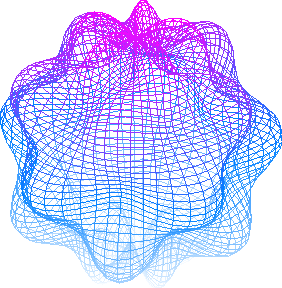
\includegraphics{poster-cover2.pdf}};
%		\node[opacity=1] at (0,-.3) {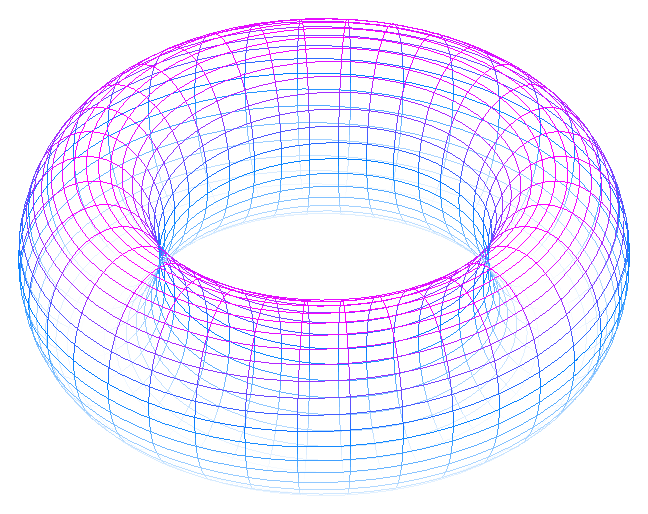
\includegraphics[scale=.5]{poster-cover3.pdf}};
		% (Optional) If you want text on the bottom arc, you can do something similar
		 \path[
		   decoration={
			     text along path,
			     text={|\large \bfseries|Academic Year 2025-2026}, % for example
			     text align={align=center},
			     raise=0.1cm
			   },
		   decorate
		 ] (200:1.4) arc (200:340:1.4);
		
		
%		%--------------------------
%		% 3. Main Math Symbols
%		%   Place iconic math symbols around the center
%		%--------------------------
%		\node at (-0.9, 0.25)  {\large $\displaystyle \int$}; % Integral sign
%		\node at ( 0.9, 0.25)  {\large $\displaystyle \sum$}; % Summation sign
%		\node at ( 0,   0.65)  {\large $\pi$};                % Pi
%		\node at ( 0,  -0.2 )  {\large $\sqrt{x}$};           % Square root
%		
%		%--------------------------
%		% 4. Coordinate Axes
%		%--------------------------
%		\draw[->](-1,0)--(1,0)  node[right] {};
%		\draw[->](0,-1)--(0,1)  node[above] {};
		
		%--------------------------
		% 6. A Little Right Triangle
		%   to highlight geometry
		%--------------------------
%		\draw (0,0) -- (0.5,0) -- (0.5,0.4) -- cycle;
%		\node at (0.25, -0.07) {\small $a$};
%		\node at (0.55, 0.20)  {\small $b$};
%		\node at (0.28, 0.25)  {\small $c$};


%========================================================
% (3) SURROUNDING MATH ELEMENTS
%========================================================
%\node[] (zero) {};
%\node[draw, circle=1pt] (a) [above left of = zero, xshift=-.5cm, yshift=.5cm]{};
%\node[draw, circle=1pt] (b) [above right of= zero, xshift=.5cm, yshift=.5cm] {};
%\node[draw, circle=1pt] (c) [below left of= zero, xshift=-.5cm, yshift=-.5cm] {};
%\node[draw, circle=1pt] (d) [below right of= zero, xshift=.5cm, yshift=-.5cm] {};
%\draw[<->, loop, looseness=10, in=120, out=60, red] (a) to (a);
%\draw[<->, loop, looseness=10, in=120, out=60, red] (b) to (b);
%\draw[<->, loop, looseness=10, in=-120, out=-60, red] (c) to (c);
%\draw[<->, loop, looseness=10, in=-120, out=-60, red] (d) to (d);
%
%% Symmetry
%\draw[dotted,->, blue, bend left] (a) to (b);
%\draw[->, blue, bend left] (b) to (a);
%\draw[dotted,->, blue, bend left] (c) to (d);
%\draw[->, blue, bend left] (d) to (c);
%
%\draw[dotted, ->, green!75!black] (a) to (b);
%\draw[dotted, ->, green!75!black] (b) to (c);
%\draw[->, green!75!black] (a) to (c); % Transitivity implied by a -> d and d -> b
%========================================================
% (2) CENTER: FUNDAMENTAL THEOREM OF CALCULUS
%========================================================
% Place the FTC formula in the center
\node at (0,-.275) {\large $\displaystyle \mathbold{\frac{d}{dx}\!\Bigl(\int_{a}^{x} f(t)\,dt\Bigr) \;=\; f(x)}$};
\node at (0,.275) {\large $\displaystyle \mathbold{\int_{a}^{b} f'(x)\,dx \;=\; f(b)-f(a)}$};

	\end{tikzpicture}
	
\end{document}
